\documentclass[times, utf8, english, diplomski]{fer}
\usepackage{booktabs}

\begin{document}

% TODO: Navedite broj rada.
\thesisnumber{1981}

% TODO: Navedite naslov rada.
\title{Software and Hardware Architecture for Redundant Embedded Systems}

% TODO: Navedite vaše ime i prezime.
\author{Dino Šarić}

\maketitle

% Ispis stranice s napomenom o umetanju izvornika rada. Uklonite naredbu \izvornik ako želite izbaciti tu stranicu.
\izvornik

% Dodavanje zahvale ili prazne stranice. Ako ne želite dodati zahvalu, naredbu ostavite radi prazne stranice.
\zahvala{Hvala.}

\tableofcontents
\listoffigures

TODO: remove!!\cite{downes2002shortams}

\chapter*{Introduction} 

In a world with increasing number of electronic systems in hazardous environment, the correct operation of active systems is ever more important for ensuring less catastrophes. In year 2000, Air France Concorde flight crashed soon after its take-of killing 113 people, in 2005 Texas City refinery exploded killing 15 people and injuring 180. Similar disasters to these were the motivation for the  creation of functional safety principles. 
\begin{figure}[H]
    \centering
    \begin{minipage}{.5\textwidth}
          \centering
          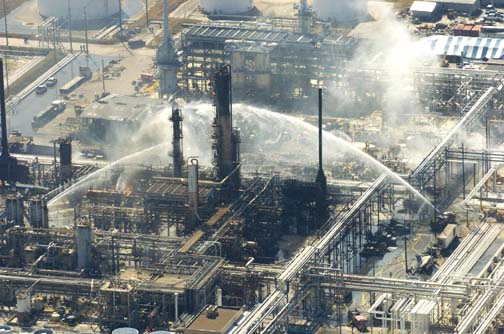
\includegraphics[width=.7\linewidth]{images/texas_refinery.jpg}
          \captionof{figure}{Texas refinery disaster}
          \label{fig:texas_refinery}
    \end{minipage}%
    \begin{minipage}{.5\textwidth}
          \centering
          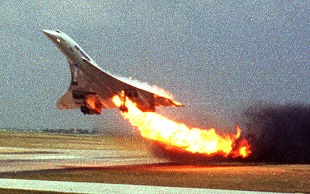
\includegraphics[width=.74\linewidth]{images/concorde_disaster.jpg}
          \captionof{figure}{ Air France Concorde disaster}
          \label{fig:concorde_disaster}
    \end{minipage}
\end{figure}

Functional safety is the part of the overall safety that depends on a system or equipment operating correctly in response to its inputs.\cite{func_safety_brief} In other words, the goal of functional safety is ensuring even when the system fails its response is predictable and safe. Today, the concept of functional safety is part of everyday life and applies to every industry one can think of. For example, functional safety ensures that airbags in a car instantly deploy during impact to protect the passengers. Another good example is an automated flight control system in the airplanes. Autopilot controls pitch and roll of the aircraft changing the heading and altitude, all of which is developed with respect to functional safety parameters, activating alarms and other measures when they are breached.\cite{func_safety_brief}

Motivation of this paper is exploring how are principles of functional safety applied to the engineering projects. Investigate how and why redundancy is implemented in hardware and software. As a part of that, redundant microcontrollers are explored and compared to non-redundant counterparts. Additionally, functional safety additions to FreeRTOS operating system are implemented. Modifications add task replication and a option to measure execution time of tasks. Finally, secure bootloader is added, bootloader has a command shell interface and has option of updating the current application.

The thesis is organized in the following way:

\begin{itemize}

    \item \autoref{functional_safety} gives brief introduction of functional safety process. Moreover, chapter gives a overview of how is hardware of embedded systems designed to support redundancy,
    \item \autoref{cortex_r_additions} investigates ARM Cortex R microcontroller's inner workings and what do they add over Cortex M,
    \item \autoref{freertos_kernel} gives overview of of FreeRTOS and inner workings of tasks, scheduler and timers,
    \item \autoref{freertos_modification} gives overview of added safety functions to the FreeRTOS kernel,
    \item \autoref{custom_bootloader} explains how the developed secure bootloader functions and its features and
    \item \autoref{demonstration} demonstrates the functionality of the developed software.
    
\end{itemize}
   
\chapter{Conclusion}

This thesis explores the functional safety practices in embedded systems. Overview of functional safety and related standards is provided to help engineers without functional safety experience. The thesis clarifies how ARM Cortex R improves functional safety principles over ARM Cortex M. 

A software is developed to achieve software redundancy in ARM Cortex M. Implemented software includes a bootloader and a modified FreeRTOS operating system.  The bootloader has the ability to load new applications and other memory manipulation related operations. The bootloader also supports permanent memory for communication between bootloader and the current application. To aid security for loading of a  new application support for HEX and SREC format is provided, along with additional checksum appended to the data.

The modified FreeRTOS operating system provides features of tracking the individual tasks execution time and task replication. Tasks tracking their time have two timers, one for overrun and one for overflow. Overrun timers count only when task is active. Overflow timer always counts regardless of the task's state. Replicated tasks can have two or three redundant tasks, when three tasks are used replicated task is fault tolerant. Demonstratration of the functionality is available through examples in source code. Inner workings of FreeRTOS and the bootloader is provided in this thesis.

\bibliography{literatura}
\bibliographystyle{fer}

% TODO: Navedite naslov na engleskom jeziku.
\begin{abstract}
Abstract.

\keywords{Keywords.}
\end{abstract}

\hrtitle{Programska i sklopovska arhitektura redundantnih ugradbenih računalnih sustava}
\begin{sazetak}
Sažetak.

\kljucnerijeci{Ključne riječi, odvojene zarezima.}
\end{sazetak}



\end{document}
